\chapter{Concepts \& Technical Implementation}
This chapter provides a detailed look at the required concepts and the technical implementation of the PWA. The project has been open-sourced to allow verification of the results\footnote{https://github.com/gunharth/bwm}. Further, the application is available online\footnote{https://bwm.gunicode.com}.

\section{Requirements}

The following section outlines the concepts and requirements used for the project by looking at the core functionality of the original \textit{Beer with Me} app.

\textbf{Progressive Web App}. The functional clone of the \textit{Beer with Me} app must implement all relevant techniques as outlined by the Progressive Web App specifications. Technologies include Service Workers, Application Shell (AppShell), Web App Manifest and serving the demo installation over HTTPS. Further, it is the intention to follow the 10 principal concepts, which lay the foundation for Progressive Web Applications, as closely as possible: Progressive, Responsive, Installable, Connectivity Independent, App-Like, Fresh, Safe, Discoverable, Re-engageable and Linkable \citep{osmaniGettingStartedProgressive2015}.

\textbf{Authentication and Authorization}. Users must be able to register for the service with a combination of E-Mail and Password. As an alternative an existing Google account may be used in order to login directly.

\textbf{Realtime Database}. Data is stored as JSON in a NoSQL database and synchronized in realtime to every connected client.

\textbf{Realtime Notifications}. If enabled by the user Push-notifications shall be sent to the user in realtime, whenever a new user registers for the service, or when a new post was published by a user.

\textbf{Realtime Map}. If enabled by the user the current geolocation of the user is saved and displayed on an online map.

\textbf{Single Page App (SPA)}. As part of this study it was my goal to implement the application as a Single Page App using one of the main JavaScrip frameworks.

Option to add a photo using the device’s camera


Frontend, Backend framework/system
straight forward deployment process

As part of this study the following points were defined as being not part of the requirements, as they do not have an impact on the used technologies of the PWA, nor do they support the output of this research. Design considerations of the application can be neglected, nor is the intention to copy the interface and design of the original \textit{Beer with Me} app. The resulting PWA focusses on the implementation of the functionality, and not to offer a duplication of the original. Further, all functions are implemented as a proof-of-concept. Thus, to make it a production ready PWA certain functionality is not implemented, like the creation of groups. The PWA supports one group only for testing purposes.


\section{Technical Implementation of Requirements}
As per the actual implementation of the PWA the goal was to base the solution on the least different providers on the one hand, as well as a minimum in terms of coding and programming languages. Hence, the front-end of the application uses the basic building blocks of regular web sites being HTML, CSS and JavaScript. To satisfy the back-end requirements A cloud solution provider

\subsection{Single Page App (SPA) \& Progressive Web App}
For the development of the frontend the JavaScript framework Vue.js\footnote{\url{https://vuejs.org}} and its ecosystem was used. The Vue Cli\footnote{\url{https://cli.vuejs.org}} offers great tooling support for Vue.js developments - among other it comes with a preset for installing a Progressive Web App skeleton.

\begin{lstlisting}[language=bash, caption=Installation and project creation commands with the Vue Cli, label=lst:vue-cli]
  $ npm install -g @vue/cli
  $ vue create beerwithme
\end{lstlisting}

On project creation Vue Cli offers you to manually select the features that will be installed. Next to Progressive Web Application support the Vue Router and Vuex was installed. The Router enables navigation services within a SPA and Vuex is responsible for the management of state within the application.

\fig{img/vue_project_creation}{Installation options for a Vue.js project}{fig:vue-project-creation}{1}

The Vue Cli PWA support comes with Workbox\footnote{\url{https://developers.google.com/web/tools/workbox}} installed - a library developed by Google for adding offline support to web applications. Among other features it mainly helps with the automatic creation and management of application caches, service worker and the creation of the web manifest for a production environment.

\begin{lstlisting}[language=JavaScript, caption=registerServiceWorker.js: Workbox registering the service worker for production, label=lst:workbox]
import { register } from "register-service-worker";
if (process.env.NODE_ENV === "production") {
  register(`${process.env.BASE_URL}firebase-messaging-sw.js`, {
    ready() {
      console.log(
        "App is being served from cache by a service worker.\n" +
          "For more details, visit https://goo.gl/AFskqB"
      );
    },
    registered() {
      console.log("Service worker has been registered.");
    },
    cached() {
      console.log("Content has been cached for offline use.");
    },
    updatefound() {
      console.log("New content is downloading.");
    },
    updated() {
      console.log("New content is available; please refresh.");
    },
    offline() {
      console.log(
        "No internet connection found. App is running in offline mode."
      );
    },
    error(error) {
      console.error("Error during service worker registration:", error);
    }
  });
}
\end{lstlisting}

The final lighthouse report for the \textit{Beer with Me PWA}:
\fig{img/lighthouse_test}{Lighthouse PWA report}{fig:lighthouse}{1}

For the front-end design of the app Vuetify\footnote{\url{https://vuetifyjs.com}} was implemented. A design component framework for Vue.js based on the material design\footnote{\url{https://material.io}} guidelines developed by Google.

\begin{lstlisting}[language=bash, caption=Command to add Vuetify to the Vue.js project, label=lst:vuetify]
  $ vue add vuetify
\end{lstlisting}

The map functionality was implemented by using the npm package vue2-leaflet\footnote{\url{https://www.npmjs.com/package/vue2-leaflet}}, which is a Vue wrapper library for the open-source JavaScript library Leaflet\footnote{\url{https://leafletjs.com}}. Map tiles are served from OpenStreetMap\footnote{\url{https://www.openstreetmap.org}}.

\begin{figure}
  \centering
  \begin{subfigure}{.5\textwidth}
    \centering
    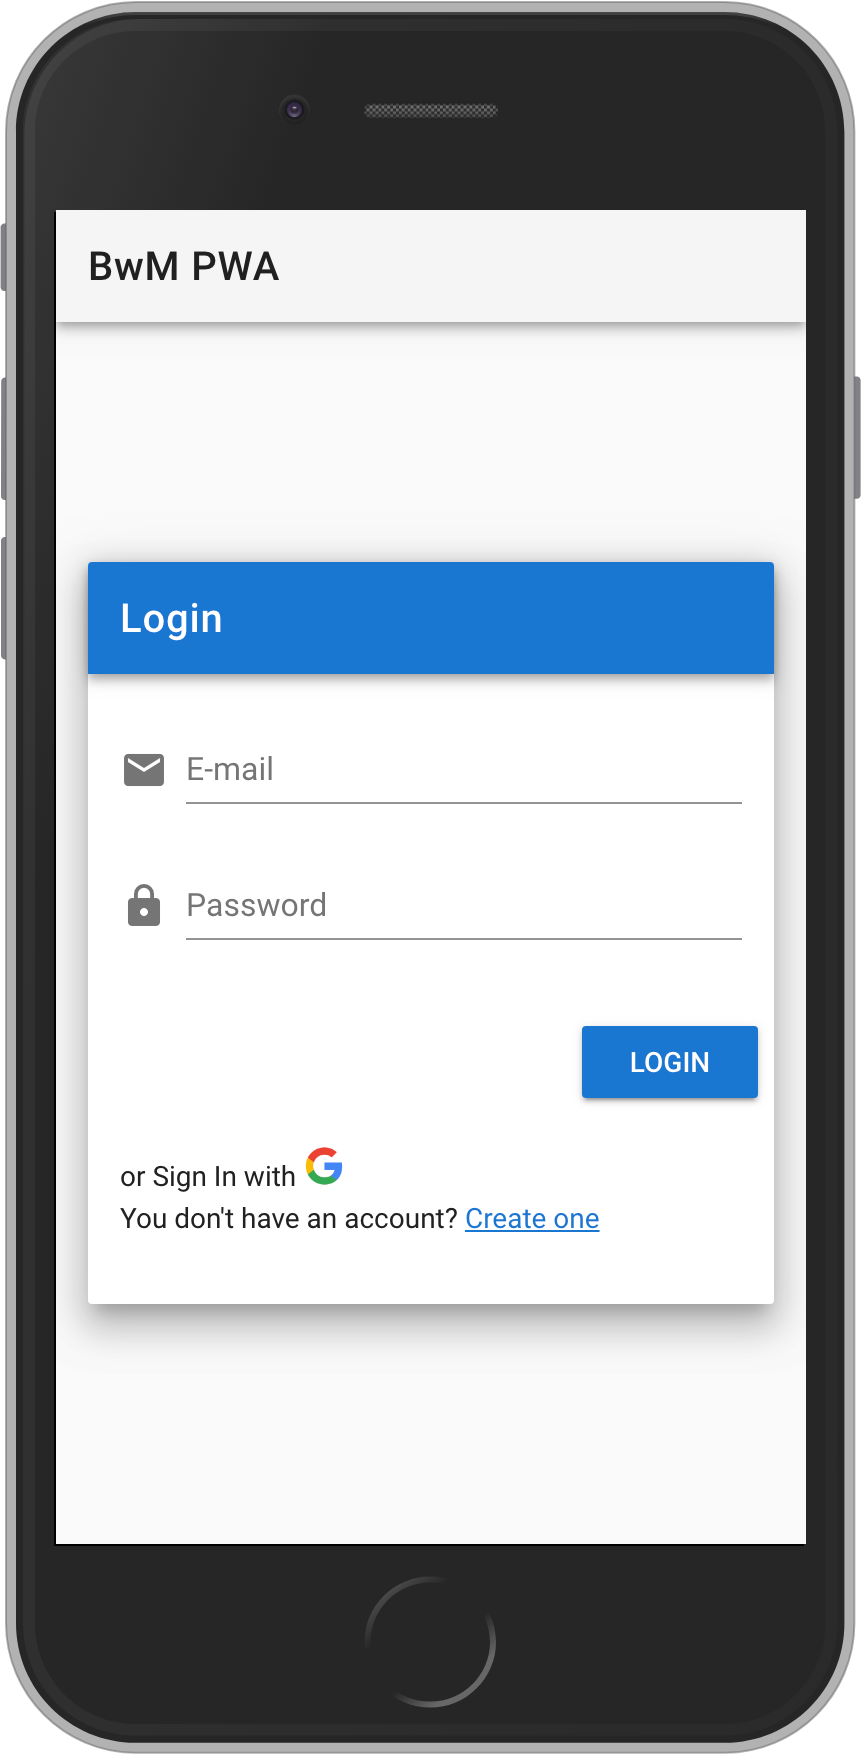
\includegraphics[width=.7\linewidth]{img/screen01}
    \caption{Login screen}
    \label{fig:sub1}
  \end{subfigure}%
  \begin{subfigure}{.5\textwidth}
    \centering
    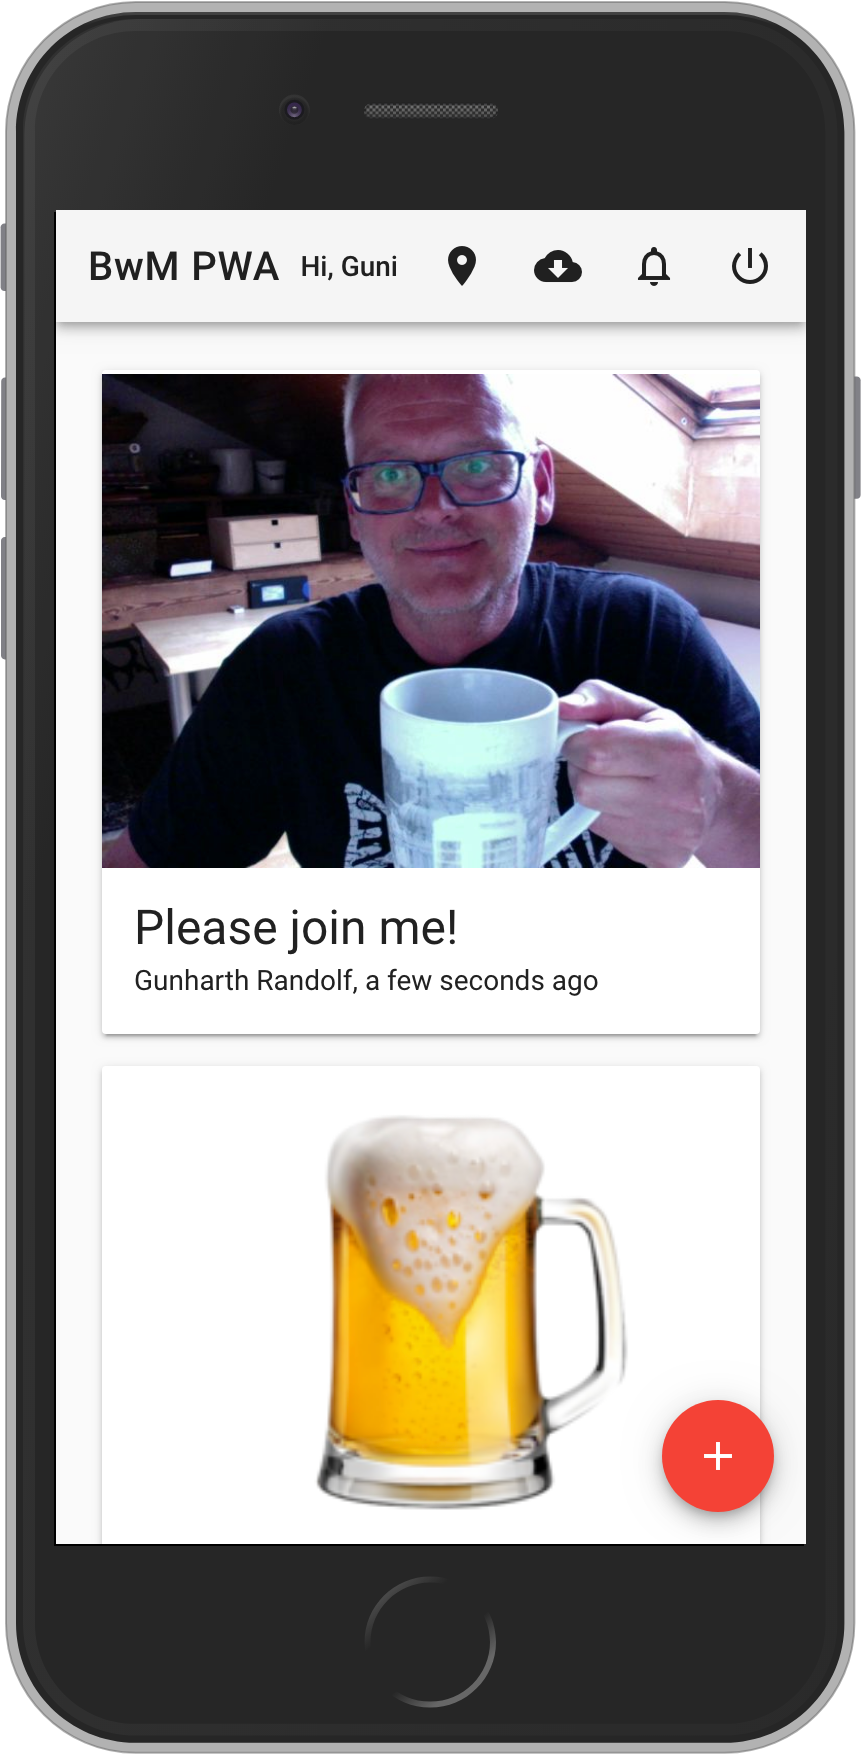
\includegraphics[width=.7\linewidth]{img/screen02}
    \caption{Main app screen}
    \label{fig:sub2}
  \end{subfigure}
  \begin{subfigure}{.5\textwidth}
    \centering
    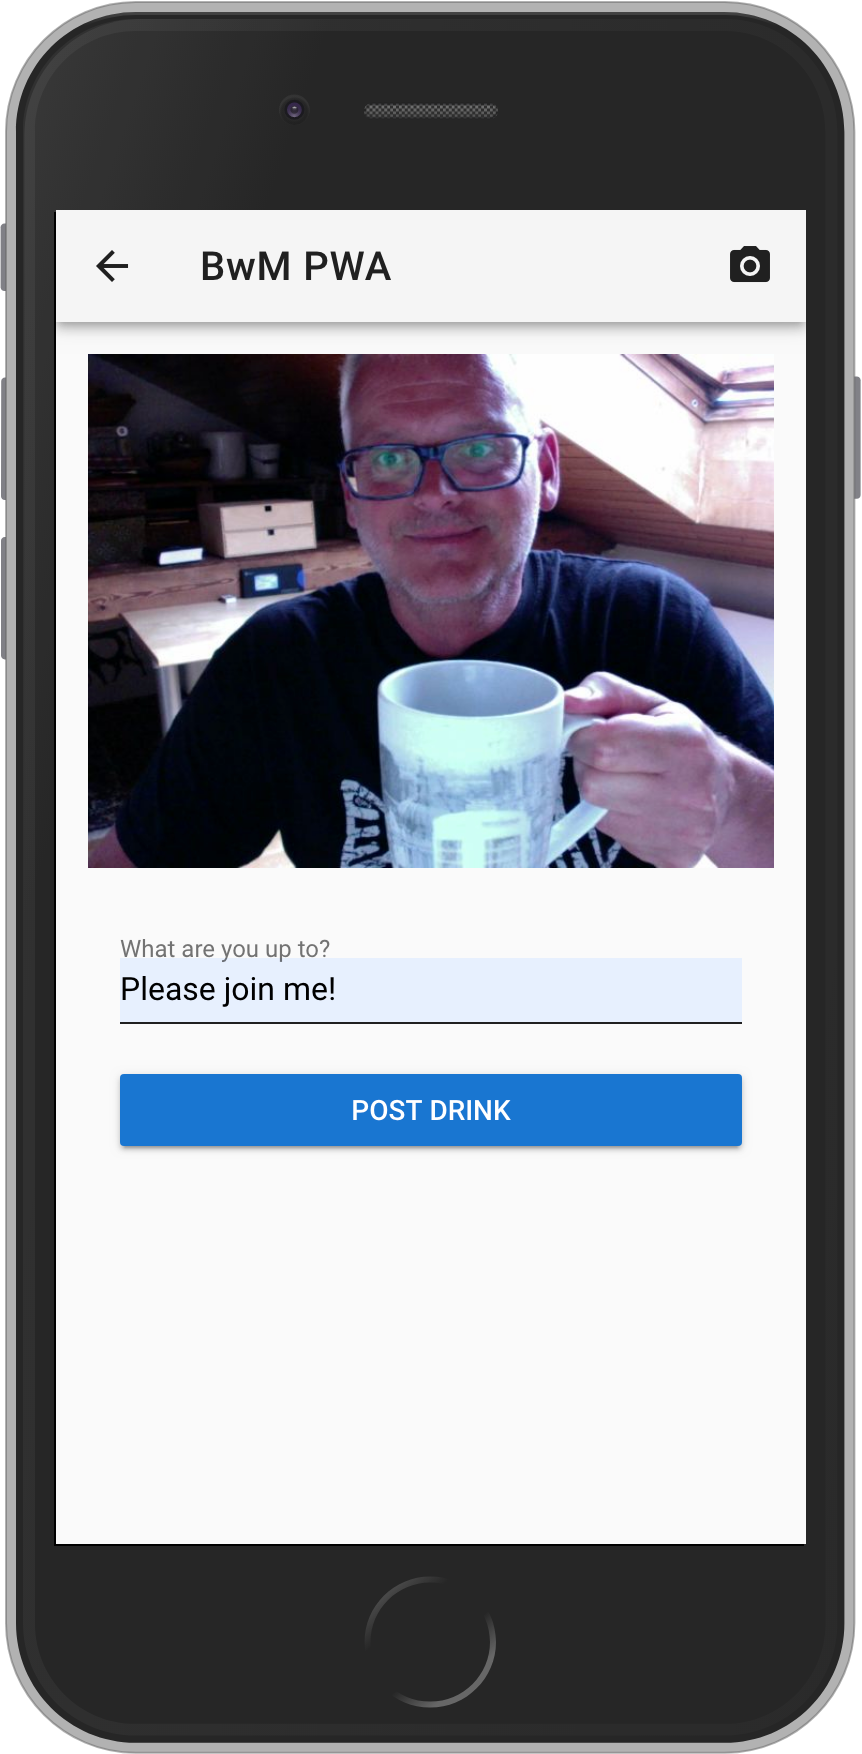
\includegraphics[width=.7\linewidth]{img/screen04}
    \caption{New post screen with photo option}
    \label{fig:sub1}
  \end{subfigure}%
  \begin{subfigure}{.5\textwidth}
    \centering
    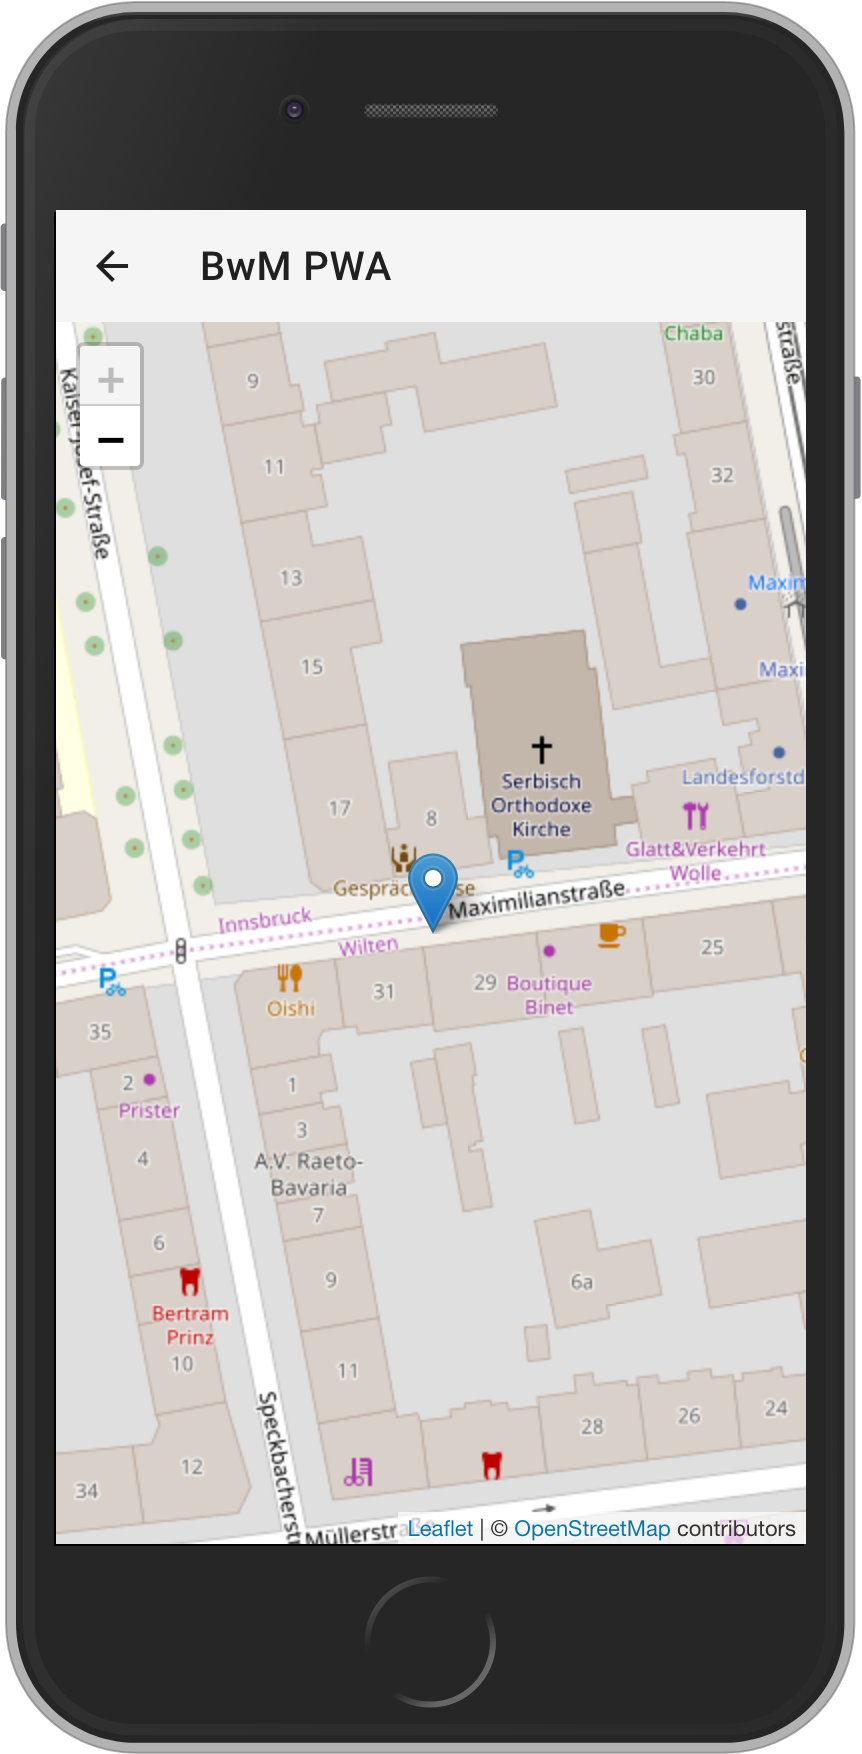
\includegraphics[width=.7\linewidth]{img/screen03}
    \caption{The map}
    \label{fig:sub2}
  \end{subfigure}
  \caption{Screenshots showing Vuetifys' material design components}
  \label{fig:test}
\end{figure}


\subsection{Cloud Provider and Realtime Functionalities}

For the purpose of the backend requirements Firebase was used. Google aquired it in 2015 ...
The Firebase service offers the following services that are required for the Beer with me project: Authentication and Authorization, Firestore offers a real time database

Authentication and Authorization

\begin{lstlisting}[language=JavaScript, caption=main.js: Firebase Auth initiation using VueJS, label=lst:firebase-auth]
  // Init firebase auth before Vue inits the App
  firebase.auth.onAuthStateChanged(firebaseUser => {
    if (firebaseUser) {
      store.dispatch("autoSignIn", firebaseUser);
    }
    if (!app) {
      app = new Vue({
        router,
        store,
        render: h => h(App)
      }).$mount("#app");
    }
  });
\end{lstlisting}

Realtime Database feeding the feed of posts on the main application page. Map positions

\begin{lstlisting}[language=JavaScript, caption=Realtime query for new posts (Home.vue), label=lst:firebase-listposts]
firebase.db
  .collection("drinks")
  .orderBy("created_at", "desc")
  .onSnapshot(snapShot => {
    this.drinks = [];
    snapShot.forEach(drink => {
      this.drinks.push({
        id: drink.id,
        url: drink.data().url,
        comment: drink.data().comment,
        author: drink.data().author,
        created_at: drink.data().created_at,
      });
    });
  });
\end{lstlisting}

Realtime Push Notifications

\textbf{Firebase}. Firebase is a service that Google aquired in 2015 ties in hand in hand with their goal on pushing on
